\subsection{Implementation}
Our framework is implemented with Pytorch. We used AES-GCM-128 as the authenticated encryption algorithm as Bonawitz etc. did\cite{Practical}. We adopted Mnist and Cifar as datasets, which is also used in the original FedAvg\cite{mcmahan2016communicationefficient}. We trained simple convolutional neural networks for the classification task. Our experiments are carried on a PC with an Intel i7-8700 CPU (3.2GHz), 16 GB of RAM, and a GTX 1080 GPU. The model was executed in a single thread to facilitate comparing and analyzing. The optimizer was stochastic gradient descent (SGD) and the learning rate is $0.01$. The $fraction$ is set as $0.1$ which means that $10\%$ of clients will be chosen to carry on the training process in each epoch.


\subsection{Accuracy}
Although our work does not modify the learning module compared to other federated learning frameworks, we still conducted a series of experiments to observe the accuracy. We compared FedAvg with our framwork on both independently identically distribution (iid) data and non-iid data to verify the effectivity. Since this experiment aims to prove the validity instead of high accuracy, the models were not trained to a high accuracy. Figure~\ref{acc} shows the result. With iid data our framework obtains accuracy quite similar with FedAvg. With non-iid data, the two systems did not match as well as they were with iid data when the $epoch$ was small. However, they finally converged to the same stable scope with the same speed, which confirmed the differences were caused by biases. Therefore, our framework changes nothing about the federated learning and it only provides privacy and robustness. 

\begin{figure}[!ht]
    \centering
    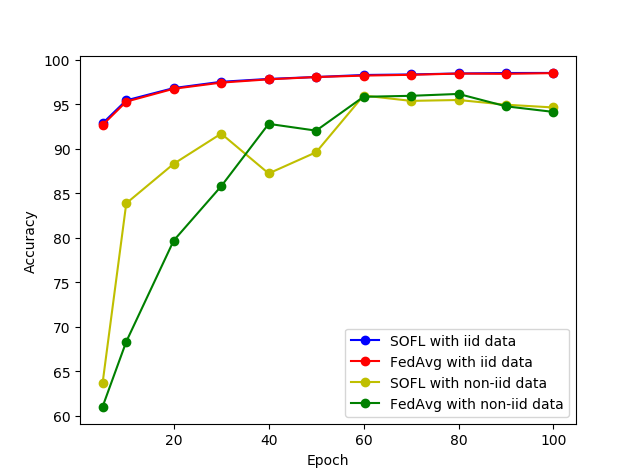
\includegraphics[width=\columnwidth]{img/acc.png}
    \caption{The accuracy of FedAvg and SOFL with iid and non-iid data in MNIST dataset. The horizontal axis $epoch$ means the total rounds that the federated learning system has been trained for.}
    \label{acc}
\end{figure}

\begin{figure}[!ht]
    \centering
    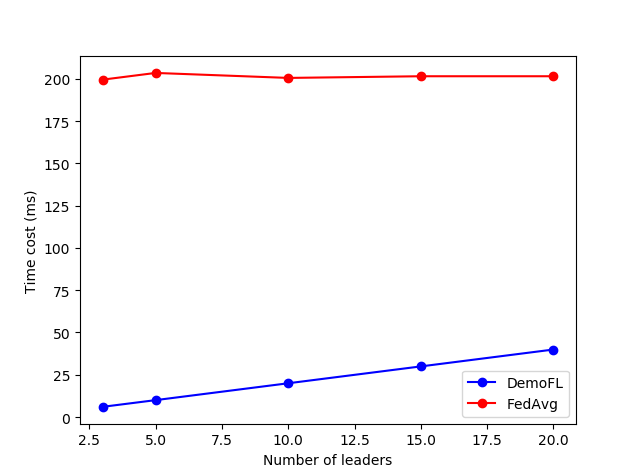
\includegraphics[width=\columnwidth]{img/leader-time.png}
    \caption{Total time spent on computation for DH protocols of FedAvg and SOFL. The number of clients is set as 100.}
    \label{leader-time}
\end{figure}

\subsection{Set-up Overhead}
In the set-up phase, our system selects several clients as leaders, and the number of leaders impacts the efficiency and a particular leader's load. We set the number of clients as $100$, and Figure~\ref{leader-time} shows the linear relation between computation time spent on diffie hellman key-exchange protocols and the number of leaders. The time spent on computation for DH protocols can be ignored compared to the learning process due to its low cost.

Meanwhile, with more leaders, one common client needs to store more keys for leaders. Apparently, the relation between number of leaders and one client's storage overhead is also linear. In addition, we can consider that in the key-exchange process of Bonawitz etc.\cite{Practical}'s system, all common clients are leaders, which requires all client-pairs to exchange keys and results in high overhead. The set-up overhead is also illustrated in Figure~\ref{leader-time}. Since it has no leaders, the computation cost does not change. Method of Kanagavelu etc.\cite{Two-Phase} performs the same as FedAvg because they did not take advantage of the server. Therefore, employing less leaders can help improving the efficiency. In contrast, employing more leaders can are beneficial to robustness because it is more flexible for t-out-of-n secret sharing methods, which we will discuss later. 


\subsection{Efficiency}
As introduced before, the additional computation insignificant compared to the communication overhead. Since the communication cost varies with equipment and environments, it is more sufficient to measure the overhead using the amount of communications instead of wall clock time. Note that a communication in our simulation means two communications in practice: a client needs to send message to the server first, and the server forwards the message to the corresponding leader. We fixed the number of leaders to 3. The amount of communications increases with the $epoch$, and the result is displayed in Figure~\ref{comm-epoch} with the assumption that there is no dropout of packets. The number of clients is another factor that impacts the efficiency. We conducted experiments with the $epoch$ set to 30 and got the results shown in Figure~\ref{comm-client}. The result is the same as what we analysed in Section IV, which means they are all of linear time complexity. Although the number of leaders also has influence on the number of communications, we did not conduct corresponding experiments because it is always set as a very small number. 


\begin{figure}[!ht]
    \centering
    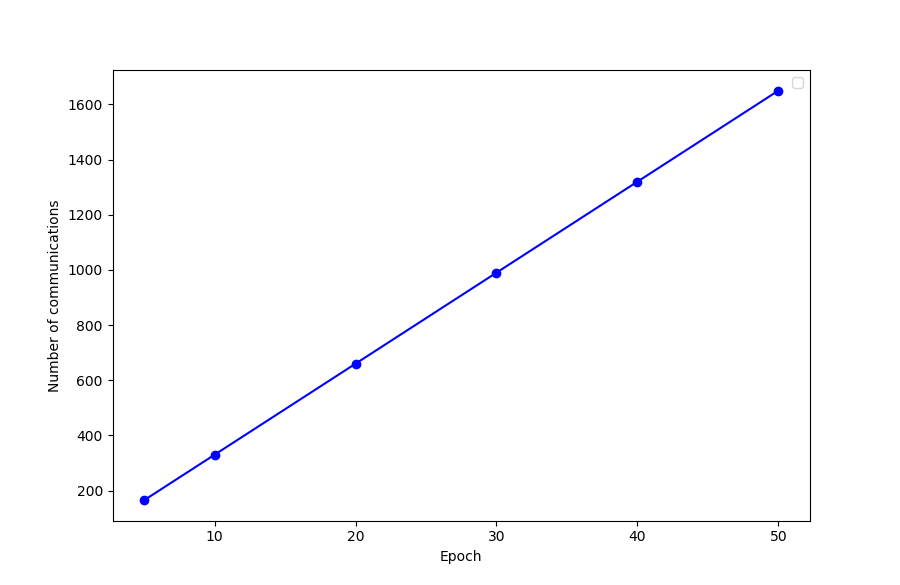
\includegraphics[width=\columnwidth]{img/comm-epoch.png}
    \caption{The amount of communications in learning process with 100 clients. The situation is without dropout.}
    \label{comm-epoch}
\end{figure}

\begin{figure}[!ht]
    \centering
    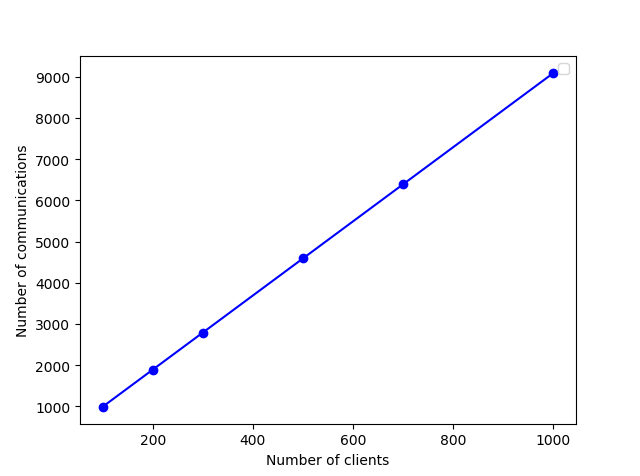
\includegraphics[width=\columnwidth]{img/comm-client.png}
    \caption{The amount of communications in learning process varies with amount of clients. The $max-epoch$ is 30 and there is no dropout.}
    \label{comm-client}
\end{figure}


\subsection{Robustness}
Our robustness is based on the re-organizing process, which happens when a leader is crashed. Crashes can hardly be avoided. Therefore, we introduced $crash_rate$, which is the possibility of that a leader would crash during one epoch, to help measuring the robustness. Generally, we consider $crash_rate$ is quite small because real crashes rarely happen in nowaday smart devices/servers. However, compared to real crashes, a leader is more likely to be unavailable due to various reasons, which also seldom happen. Therefore we still consider $crash_rate$ would not be larger than $0.1$. We conducted several experiments to how $crash_rate$ impacts the efficiency. First, we set the number of clients to 100 and the $max-epoch$ to 10. Figure~\ref{comm-crash} shows that when crashes happened, it impacts the same on the value of communications instead of the ratio despite of the $epoch$. E.g., a crash with $epoch$ 10 resulted in $66\%$ overhead approximately and it only resulted in about $0.06\%$ overhead when the $epoch$ is $100$. It indicates that a high $crash_rate$ does impact the efficiency heavily when $epoch$ is low. However, when the $epoch$ gets larger, the influence of crashes becomes insignificant. Considering that the $epoch$s used in real federated learning works are quite large, SOFL provides sufficient efficiency and robustness.

\begin{figure}[!ht]
    \centering
    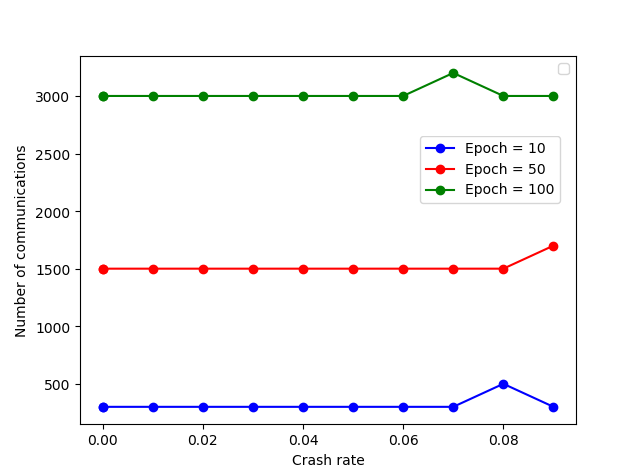
\includegraphics[width=\columnwidth]{img/comm-crash.png}
    \caption{The average amount of communications with different crash rates.}
    \label{comm-crash}
\end{figure}

